\subsection{Теоретическое введение и методы}

\paragraph{Линейная некогерентная система}
Пусть оптическая система имеет входную и выходную плоскости, на входной плоскости задаётся некоторое поле, а на выходной -- регистрируется. Если в этой системе отсутствуют нелинейные элементы, то поле на выходе этой системы в зависимости от входного поля представимо через функцию Грина \cite{MMF}, это показано в уравнении \ref{eq:FieldGrinFunc}. В выражениях опущена зависимость от времени, так как поле монохроматично и эту зависимость можно выразить через комплексную экспоненту, которая в силу линейности выносится за скобки во всех уравнениях.
\begin{equation}\label{eq:FieldGrinFunc}
	E_2(x,y) = \int\limits_{-\infty}^{+\infty}\int\limits_{-\infty}^{+\infty}E_1(\tilde{x},\tilde{y})G(x,y,\tilde{x},\tilde{y})d\tilde{x}d\tilde{y}.
\end{equation}
Физический смысл функции Грина заключается в отклике системы на точечный источник в координате $\tilde{x},\tilde{y}$ входной плоскости. Само выражение представляет суперпозицию откликов от всех точек. Пусть поле имеет некоторую пространственную некогерентность, тогда амплитуда входного поля $E_1(x,y)$ становится случайной величиной. Пусть на выходной плоскости представляет интерес только интенсивность поля, выражаемая уравнением \ref{eq:Int0}, это предположение логично, потому что оптические детекторы могут измерять только интенсивность.
\begin{equation}\label{eq:Int0}
	I(x,y) = \frac{c}{4\pi}\left<\left|E_2(x,y)\right|^2\right> = \frac{c}{4\pi}E_2(x,y)E_2^*(x,y).
\end{equation}
Комплексное сопряжение внесено под интеграл в силу его линейности, поэтому выражение для интенсивности выглядит принимает вид, смотреть уравнение \ref{eq:Int1}:
\begin{equation}\label{eq:Int1}
	\begin{gathered}
		I(x,y) = \\ \frac{c}{4\pi}
		\left(\int\limits_{-\infty}^{+\infty}\int\limits_{-\infty}^{+\infty}E_1(\tilde{x},\tilde{y})G(x,y,\tilde{x},\tilde{y})d\tilde{x}d\tilde{y}\right)
		\times
		\left(\int\limits_{-\infty}^{+\infty}\int\limits_{-\infty}^{+\infty}E_1^*(\tilde{x},\tilde{y})G^*(x,y,\tilde{x},\tilde{y})d\tilde{x}d\tilde{y}\right)
	\end{gathered}.
\end{equation}
Для нахождения среднего от выражения \ref{eq:Int1} по определению, необходимо учесть что подынтегральная функция зависит от случайных величин $E(\tilde{x},\tilde{y})$ во всех точках исходной плоскости. Поэтому, для её вычисления необходимо знать полную плотность вероятности. Вместо полной плотности вероятности, можно использовать вероятность конкретной реализации поля $P_n$, а саму реализацию через $E_{1,n}(\tilde{x},\tilde{y})$. Тогда, вместо интегрирования по всем возможным значениям величины поля в каждой точке, будем использовать сумму. Это выражение записано в формуле \ref{eq:Int2}.
\begin{equation}\label{eq:Int2}
	\begin{gathered}
		\left<I(x,y)\right> =
		\frac{c}{4\pi} \sum\limits_{n}P_n
		\left|\int\limits_{-\infty}^{+\infty}\int\limits_{-\infty}^{+\infty}
		E_{1,n}(\tilde{x},\tilde{y})
		G(x,y,\tilde{x},\tilde{y})d\tilde{x}d\tilde{y}\right|^2
	\end{gathered}.
\end{equation}
Обратим внимание, что выражение под модулем представляет прохождение когерентного поля $E_{1,n}(\tilde{x},\tilde{y})$ через систему с функцией Грина $G(x,y,\tilde{x},\tilde{y})$. Обозначив результат когерентного распространения как $E_{2,n}(\tilde{x},\tilde{y})$ для конкретной реализации получим:
\begin{equation}\label{eq:Int3}
	\begin{gathered}
		\left<I(x,y)\right> =
		\frac{c}{4\pi} \sum\limits_{n}P_n
		\left|
		E_{2,n}(\tilde{x},\tilde{y})
		\right|^2
	\end{gathered}.
\end{equation}
Если выбрать равновероятные реализации поля $E_{1,n}(\tilde{x},\tilde{y})$, то выражение примет вид:
\begin{equation}\label{eq:IntMain}
	\begin{gathered}
		\left<I(x,y)\right> =
		\frac{c}{4\pi} \lim\limits_{N \rightarrow \infty}\frac{1}{N}\sum\limits_{n=0}^{N}
		\left|E_{2,n}(\tilde{x},\tilde{y})\right|^2
	\end{gathered}.
\end{equation}
По сути, эта оценка аналогична оценке среднего случайной величины и стремится к реальному среднему при стремление $N$ к бесконечности.



\paragraph{Генерация реализаций некогерентного поля}
Для генерации реализаций некогерентного поля необходимо знать, в общем случае, полную совместную плотность вероятности поля в каждой точке. Эта функция имеет неограниченное количество аргументов. После дискретизации системы на расчётную сетку, количество точек входной плоскости системы станет ограниченным и, теоретически, такую функция можно задать. Однако, количество данных, которые будет необходимо хранить будет пропорционально $N^N$, где $N$ -- количество узлов в начальной плоскости. Можно попробовать ограничится некоторым приближением, которые описаны в разделе \ref{par:SpatialIncoherence}. Чтобы учесть некогерентность, как было показано в этом параграфе, необходимо брать хотя бы первое приближение. В первом приближении, количество данных, необходимых на хранение функции плотности распределения в памяти компьютера будет пропорционально $N^2$. При этом, $N$ должно быть достаточным для корректной работы численных методов, т.е. шаг сетки по каждой оси должен быть порядка длинны волны. Для расчёта поля размером $1$ мм на $1$ мм необходимо порядка $\frac{10^{-3}}{512*10^{-9}} \approx 1000$ точек по каждой оси, в итоге $N = (1000 \times 1000)^2 = 10^{12}$. Если хранить такое количество числе в формате $32$ битного числа с плавающей точкой, то такой массив займёт в памяти примерно $3.6$ ТБайта. Для современных компьютеров эта величина велика, по сравнению с размерами оперативной и/или видео памяти, которые исчисляются Байтами. Поэтому был выбран другой метод.
\par
Метод заключается в генерации случайного фазового поля и последующего подбора параметров генерации так, чтобы интересующие нас метрики имели заданные характеристики. Генерируется случайный Фурье образ, значение в каждой точке которого равновероятно может принимать значение от $0$ до $1$, и ограничивается гауссовой функцией с дисперсией $\frac{1}{\sigma^2}$. По свойству Фурье преобразования, при обратном преобразовании, характерные области похожих значений будут иметь размеры порядка $\sigma^2$. Однако, сложение множества равномерно распределённых величин при обратном преобразовании Фурье приведёт к распределению Гаусса в каждой точке фазового поля. Фаза должна являться равномерно распределённой, поэтому от полученного поля берётся функция, обеспечивающая равномерную распределённость результата. На рисунке \ref{ris:IncoherentRAD} отображены примеры генерации случайного нормализованного от $0$ до $1$ фазового поля при различных уровнях пространственной когерентности.
\begin{figure}[htbp]
	\centering{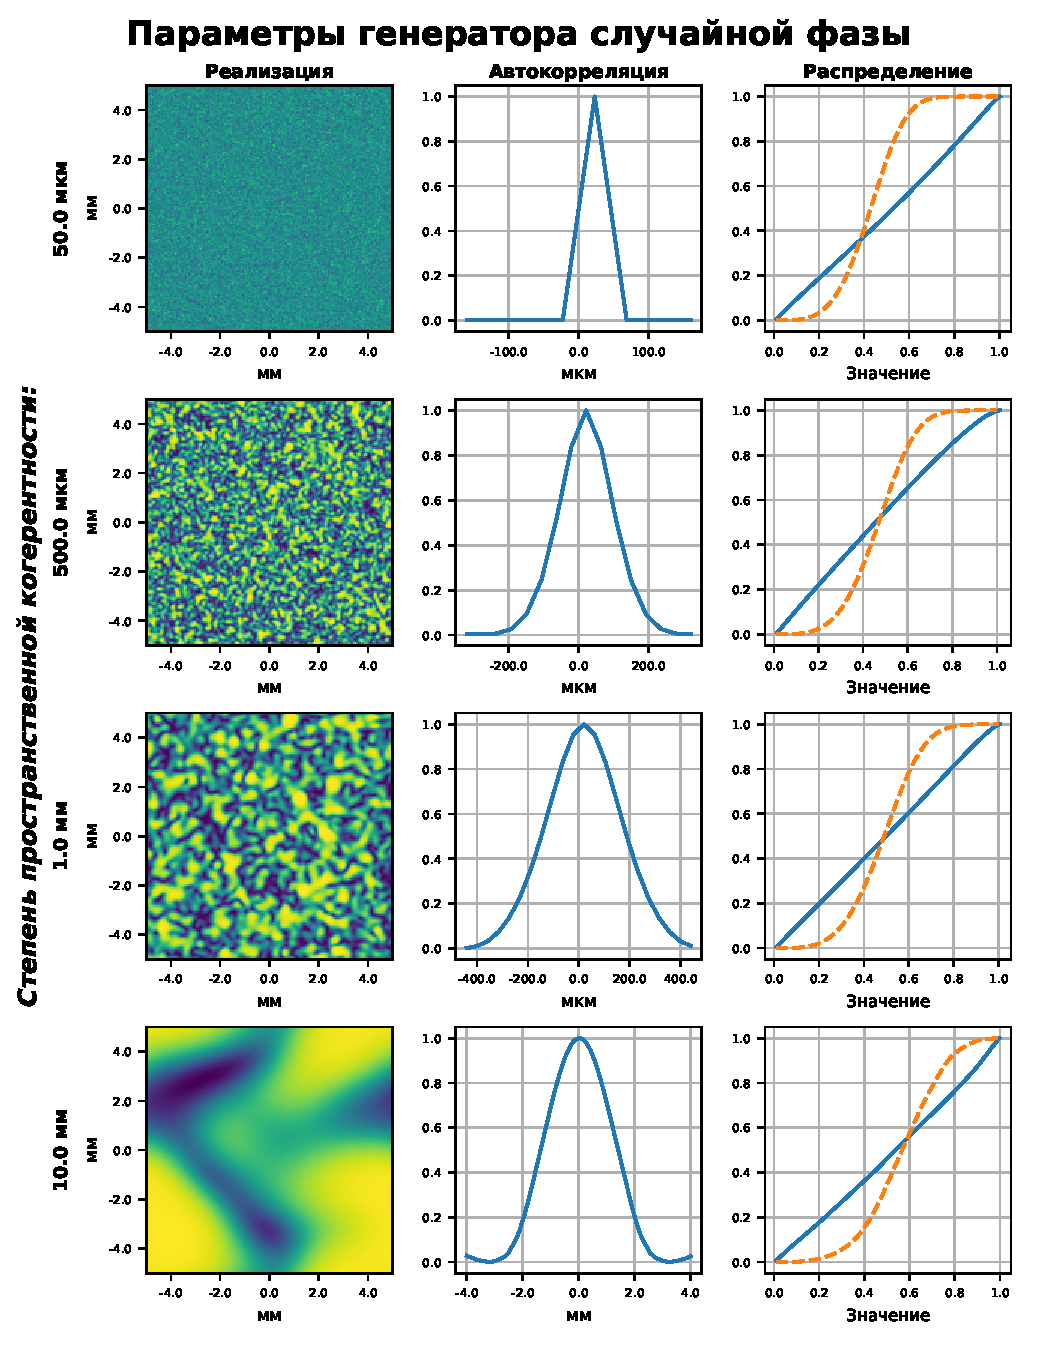
\includegraphics[width=1.0\linewidth]{figures/IncoherentRAD.eps}}
	\caption{Первая колонка -- конкретная реализация случайного поля, нормированного от $0$ до $1$, вторая -- усреднённая и нормированная автокорреляционная функция с зависимостью от радиуса, третья -- прерывистая линия изображает распределение до нормализации, сплошная -- после.}
	\label{ris:IncoherentRAD}
\end{figure}
Видно, что вычисленный размер корреляции фазы не соответствует установленному, однако величины похожи. Для точных расчётов будут подбираться параметры так, чтобы автокорреляция соответствовала реальной.


\paragraph{Прохождение света через маску}
В модели учитывается, что маска достаточно тонкая, чтобы считать, что при прохождение поле $E(x,y)$ просто умножается на функцию маски $M(x,y)$. Функция маски является суперпозицией областей. Каждая область одинаково модулирует поле в некоторой квадратной области. На каждую такую область приходится несколько точек вычислительной сетки. Это необходимо для учёта размера областей неоднородности маски.



\paragraph{Расчёт когерентного распространения}
Распространение когерентного света реализовано модифицированным методом углового спектра. Метод углового спектра заключается в представлении поля в исходной плоскости как суперпозиции трёхмерных плоских волн, распространение каждой волны на заданное расстояние $L$ и их сложение в выходной плоскости. Математически это выражение записывается следующим образом:
\begin{equation}\label{eq:ASM}
	E(x,y,L) = \mathcal{F}^{-1}\left(\mathcal{F}\left(E(x,y,0)\right)e^{ik_z(k_x,k_y)L}\right),
\end{equation}
где $\mathcal{F}$ - Фурье преобразование. Этот алгоритм использует быстрое преобразование Фурье, что делает его намного быстрее аналогов, а также сокращает размер вычислительного графа, необходимого для использования методов машинного обучения. Однако, быстрое преобразование Фурье дискретно и подразумевает периодические граничные условия, что вызывает ошибки расчёта. Способ решения этой проблемы -- добавление пустых полей на границах исходного поля, чтобы увеличить размер периодичности. Для определения размера этих полей, нужно применить теорему о свёртке к выражению \ref{eq:ASM} и получить выражение \ref{eq:ASMConv}.
\begin{equation}\label{eq:ASMConv}
	E(x,y,L) = E(x,y,0) \bullet \mathcal{F}^{-1}\left(e^{ik_z(k_x,k_y)L}\right).
\end{equation}
В этом выражение символ $\bullet$ обозначает свёртку, а $\mathcal{F}^{-1}\left(e^{ik_z(k_x,k_y)L}\right)$ называется ядром. Если интересной является некоторая область $x,y \in [0,D]$, то без полей, $E(x,y,0)$ будет периодично по двум осям с периодом $D$. Если ядро имеет такой-же характерный размер $D$, то при свёртке, на значения поля в области $x,y \in [0,D]$ будут влиять не только значения исходного поля в это области, но и значения, находящиеся за границей на расстоянии вплоть до $\frac{D}{2}$. Поэтому исходную область нужно расширять нулевыми границами на расстояние равном $\frac{D}{2}$ в каждую сторону. Рисунок \ref{ris:PropagationSlit} показывает корректность работы модели распространения. Красные линии показывают теоретически рассчитанные положения дифракционных минимумов.
\begin{figure}[htbp]
	\centering{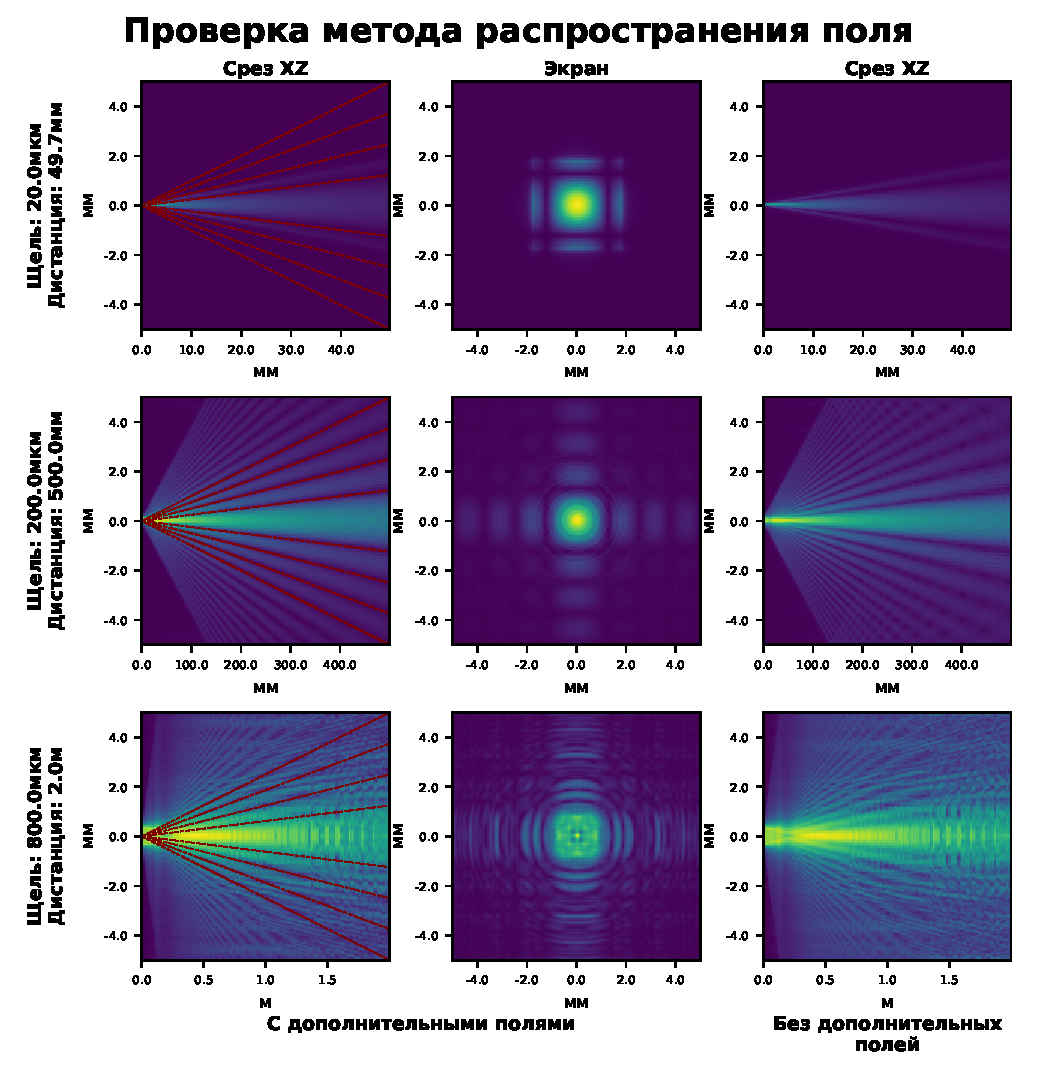
\includegraphics[width=1.0\linewidth]{figures/PropagationSlit.eps}}
	\caption{Проверка работы метода распространения некогерентного света на щелевой дифракции. Длинна волны: $500$нм.}
	\label{ris:PropagationSlit}
\end{figure}
По данному эксперименту видна необходимость модификации метода. Для этого сравним третью картинку и первую картинки во втором ряду. На третьей картинке, где для расчётов не добавляются пустые поля, видно как приходят лучи от несуществующего источника за границами области расчёта. Понятно, что если бы щель находилась на границе вычислительной области, то мнимые лучи были бы намного интенсивней, потому что приходили бы от первого дифракционного максимума мнимого источника. Также, видна необходимость использования нескольких вычислительных узлов на каждую неоднородность. В первом ряду, дифракционные максимумы обрезаются именно из-за нехватки вычислительных узлов, приходящихся на щель. В третьем ряду видно, что модель сильно шумит при больших расстояниях распространения.
\par
Полученные результаты свидетельствуют о корректности работы модели распространения когерентного света. Были получены оценки параметров, необходимых для наилучших результатов расчёта.



\paragraph{Линейная модель и некогерентный свет}
На поле в исходной плоскости линейной системы накладывается накладываются различные реализации случайной фазы. Далее, для каждой наложенной реализации, рассчитывается поле в выходной плоскости, как в когерентном случае. После этого, происходит усреднение по реализациям согласно уравнению \ref{eq:IntMain}. На рисунке \ref{ris:YungExperiment} представлены результаты расчёта опыта Юнга с учётом пространственной некогерентности света. В последней строчке этого рисунка находится график зависимости видности $\gamma$ интерференционной картины от степени когерентности $\sigma$. Уравнение \ref{eq:Visibility} представляет выражение для $\gamma$.
\begin{equation}\label{eq:Visibility}
	\gamma = \frac{I_{max}-I_{min}}{I_{max}+I_{min}}.
\end{equation}
\begin{figure}[htbp]
	\centering{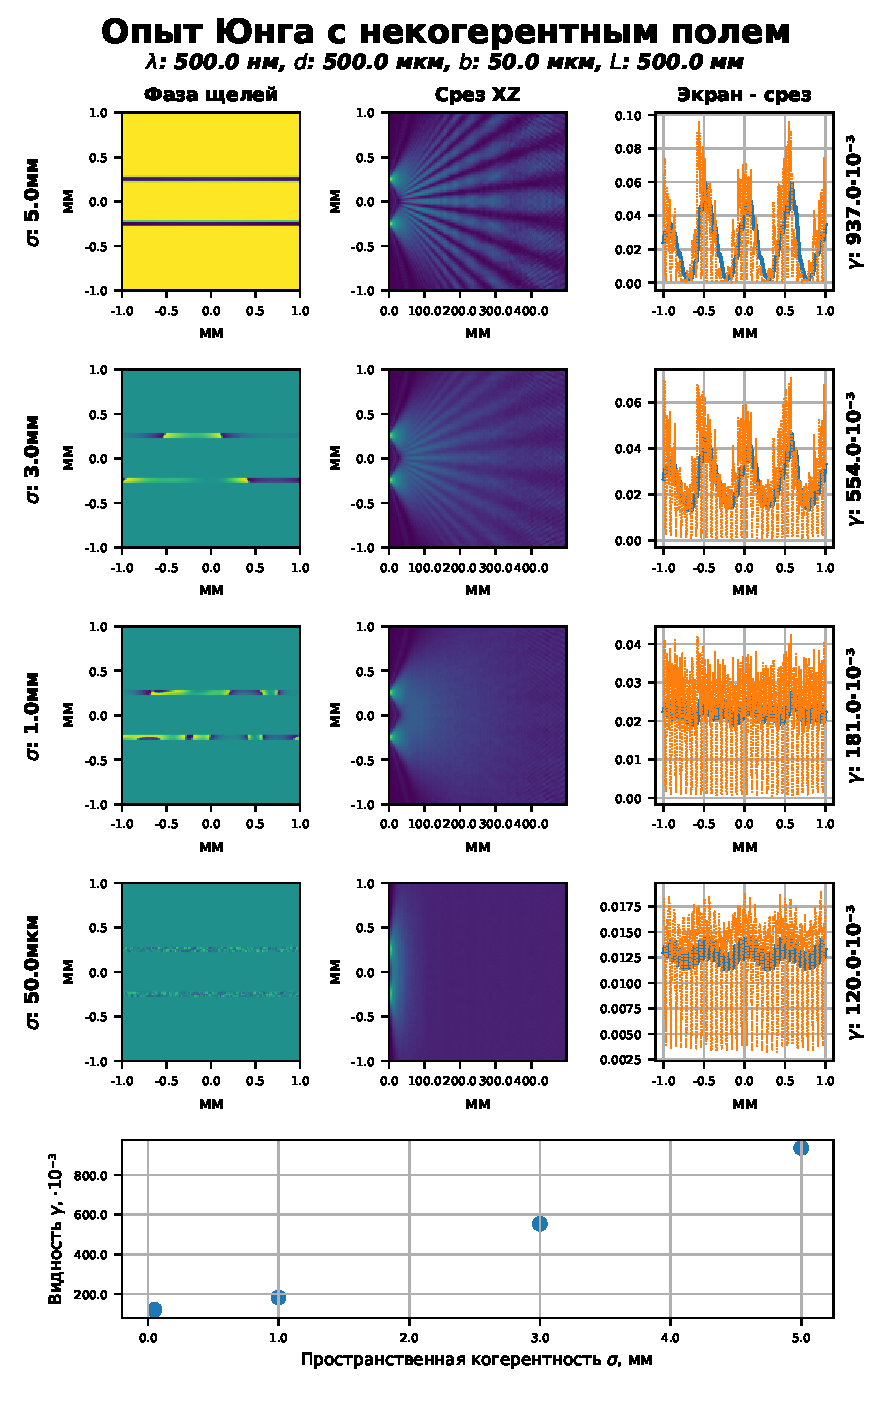
\includegraphics[width=0.95\linewidth]{figures/YungExperiment.eps}}
	\caption{$\lambda$ -- длина волны, $d$ -- расстояние между щелями, $b$ -- ширина щели, $L$ -- расстояние до экрана, $\sigma$ -- когерентность, $\gamma$ -- видность. В третьем столбце оранжевый цвет соответствует реальному результату, синий -- оконному усреднению.}
	\label{ris:YungExperiment}
\end{figure}
Система ведёт себя так, как и ожидалось от опыта Юнга в некогерентном излучении, что говорит о корректности работы метода. Другой эксперимент необходимый для верификации модели -- построение изображение в линзе, представленный на рисунке \ref{ris:Lenses}. Исходное изображение для этого эксперимента на рисунке \ref{ris:LensImage}. Линза моделировалась как тонкая маска, модулирующая фазу.
\begin{figure}[!htbp]
	\centering{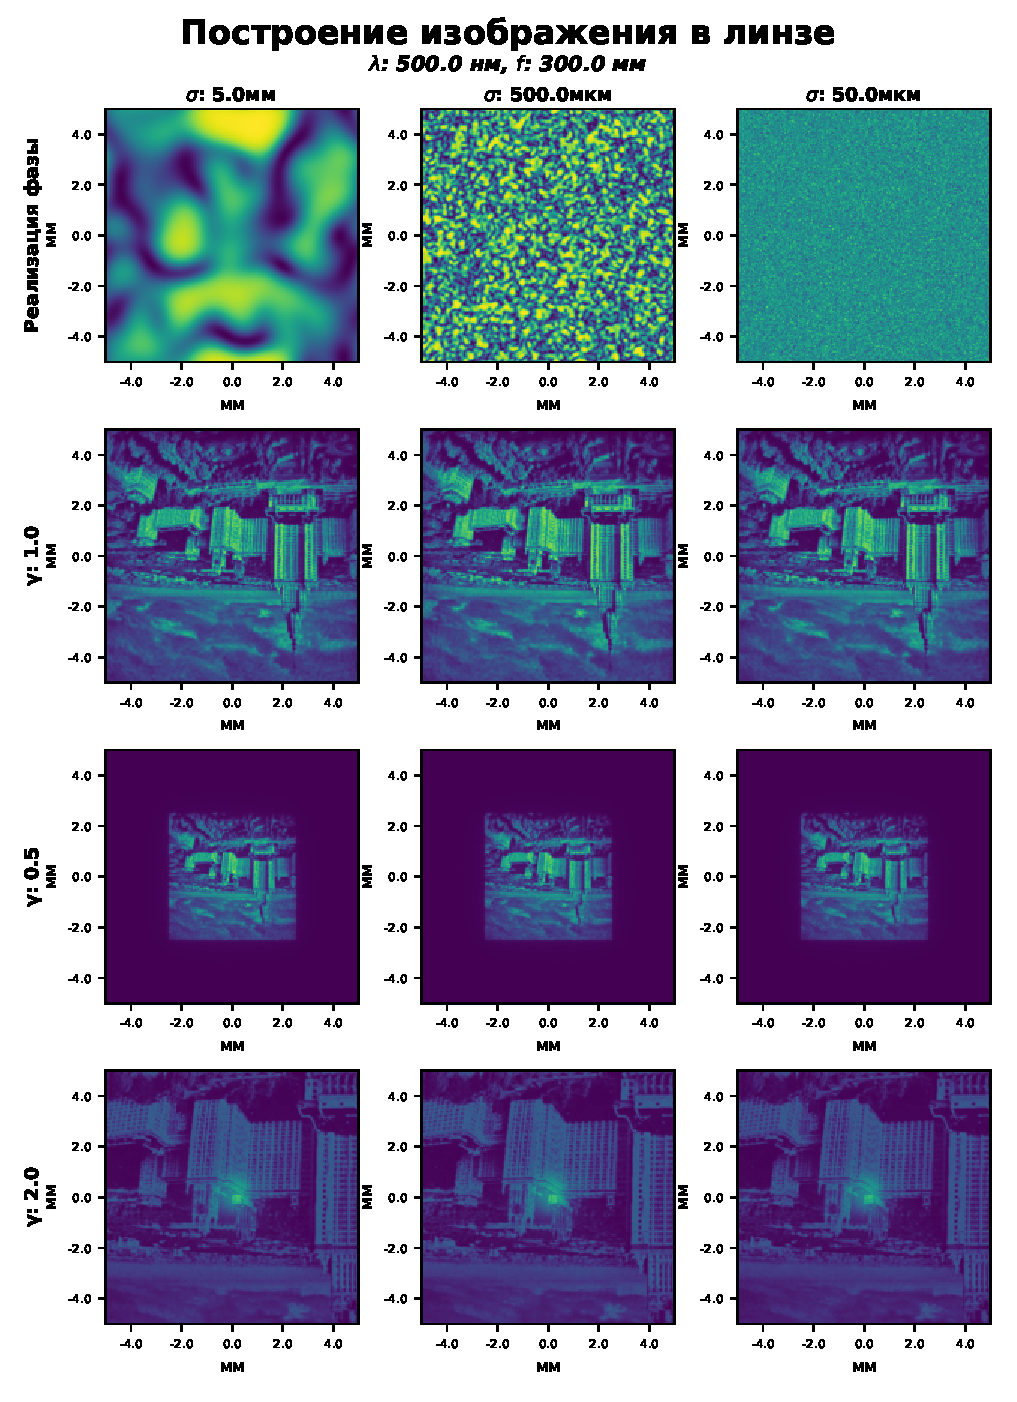
\includegraphics[width=0.95\linewidth]{figures/Lenses.eps}}
	\caption{$\lambda$ -- длина волны, $f$ -- фокусное расстояние линзы, $\sigma$ -- когерентность, $\gamma$ -- увеличение системы.}
	\label{ris:Lenses}
\end{figure}
\begin{figure}[htbp]
	\centering{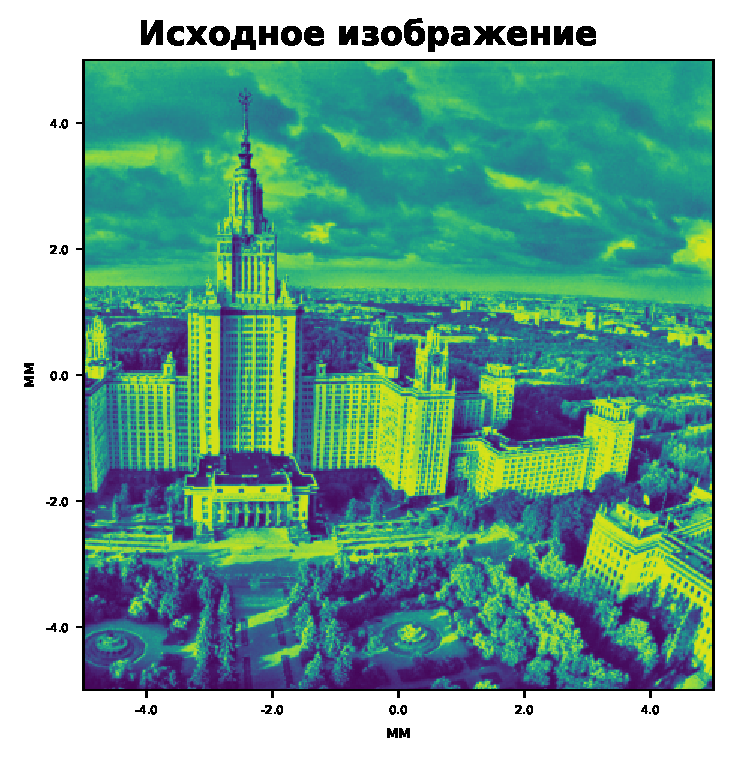
\includegraphics[width=0.5\linewidth]{figures/LensImage.eps}}
	\caption{Изображение, использованное для построения изображения в линзе.}
	\label{ris:LensImage}
\end{figure}
Видно, что в некогерентном излучении линза продолжает корректно строить изображение в различных конфигурациях. Стоит, однако, отметить, что использование линзы в системе накладывает некоторые ограничения на степень дискретизации вычислительной сетки и размер вычислительной области. Модуляция линзы между двумя точками не должна сильно изменяться. Нарушение этого правила приводит к существенным артефактам и расщеплению изображения. Ситуация усложняется тем, что скорость модуляции фазы растёт с удалением от оптической оси. В уравнении \ref{eq:LensPhase} показана дополнительная фаза, добавляемая линзой, в зависимости от координат $x,y$.
\begin{equation}\label{eq:LensPhase}
	\Delta\varphi = \pi\frac{\left(x^2 +y^2\right)}{\lambda f}.
\end{equation}
Пусть $\Delta$ -- характерная дискретизация, $M$ -- максимальный размер, тогда можно выполнить оценку связи этих величин $\Delta \le \frac{\lambda f}{4M}$. Если выразить количество вычислительных узлов по каждой оси то получится $N \ge \frac{4}{\lambda f} M^2$. Такая квадратичная зависимость	 ограничивает возможность рассчитывать большие системы. Для характерных величин $M=10$мм, $\lambda=500$нм, $f=30$см, можно получить $\Delta=3.75$мкм, т.е. для отсутствия ошибок при таких параметрах необходимо минимум примерно $2700$ точек.
